\documentclass{article}
\usepackage[a4paper, total={7.5in, 10in}]{geometry}
\geometry{paperwidth=10in, 
	%paperheight=16383pt, 
	paperheight=8100pt,
	left=2in, top=40pt, textwidth=6in, marginparsep=20pt, marginparwidth=1.5in, %textheight=16263pt, 
	textheight=8000pt,
	footskip=40pt
}
\usepackage{graphicx}
\usepackage{url}
\usepackage{natbib}
\usepackage{todonotes}
\usepackage{booktabs}
\usepackage{lineno}
\usepackage{color}
%\usepackage{auto-pst-pdf}
\usepackage[colaction]{multicol}
\usepackage{caption}
\usepackage{svg}
\usepackage{authblk}
\usepackage{standalone}
\usepackage[section]{placeins}


\linespread{1.5}

\bibliographystyle{apalike}

\makeatletter
\renewcommand{\maketitle}{\bgroup\setlength{\parindent}{0pt}
	\begin{flushleft}

		{\huge\textbf{\@title}}

		\bigskip

 		{\large\textbf{\@author}}

 		\bigskip

 		{\large{Draft current \@date}}

	\end{flushleft}\egroup
}
\makeatother

\newcommand{\multicollinenumbers}{
	\linenumbers
	\def\makeLineNumber{\docolaction
		{\makeLineNumberLeft}
		{}
		{\makeLineNumberRight}
		}
}

\newenvironment{figurehere}
	{\def\@captype{figure}}
	{}

% Title
\title{A Topic Model of Climate Change Literature}
\title{Words, words, words: Mapping the Matter of Climate Change Literature}
\title{A Topography of Climate Change Research - Results}
\author[1,2]{Max Callaghan}

\affil[1]{Mercator Research Institute on Global Commons and Climate Change, Torgauer Straße, 10829 Berlin, Germany}
\affil[2]{School of Earth and Environment, University of Leeds, Leeds LS2 9JT, United Kingdom}

\begin{document}
\maketitle

\section{Results}

\setcounter{totalnumber}{200}

\subsection{Literature growth}

The literature on climate change has grown rapidly \citep{Grieneisen2011}. The implications for the IPCC are discussed in \citep{Minx2017l}. Since that study's publication, growth has continued (see SI figure x.)

Not only are more articles being published, the range of themes being discussed in the context of climate change (see for example recently zika and biochar, which were not to be found at all before ARs 6 and 5 respectively) has expanded.
	
\begin{table}[h]
	\scriptsize
	\begin{tabular}{|l |p{1.8cm} p{1.8cm} p{1.8cm} p{1.8cm} p{1.8cm} p{1.8cm}|} 
\hline 
&\textbf{AR1} & \textbf{AR2} & \textbf{AR3} & \textbf{AR4} & \textbf{AR5} & \textbf{AR6}\\ \hline
	\caption{Growth in climate change literature}
	\label{growthtable}
\end{table}

Topic modelling helps us to map out the literature, and make sense of broad patterns in the distribution of documents and their words. In this way, we can answer questions about the growth of the climate change literature, and its representation in IPCC assessment reports. The answers to these questions can help inform IPCC processes, and understand how the IPCC functions.

%\begin{figure}[h]
%	\begin{center}
%		\includegraphics[width=0.5\linewidth]{plots/literature_size/volume_variety.pdf}
%		%\captionof{figure}
%		\caption{The volume and variety of literature on climate change has grown to unmanageable proportions. Each box represents a document-term matrix (unique documents x unique terms) of the abstracts written in each assessment period. The percentage of documents in which the average word occurs in is given in the key.
%		}
%	
%		\label{growth}
%	\end{center}
%\end{figure}



%\begin{figure}[h]
%	\begin{center}
%		%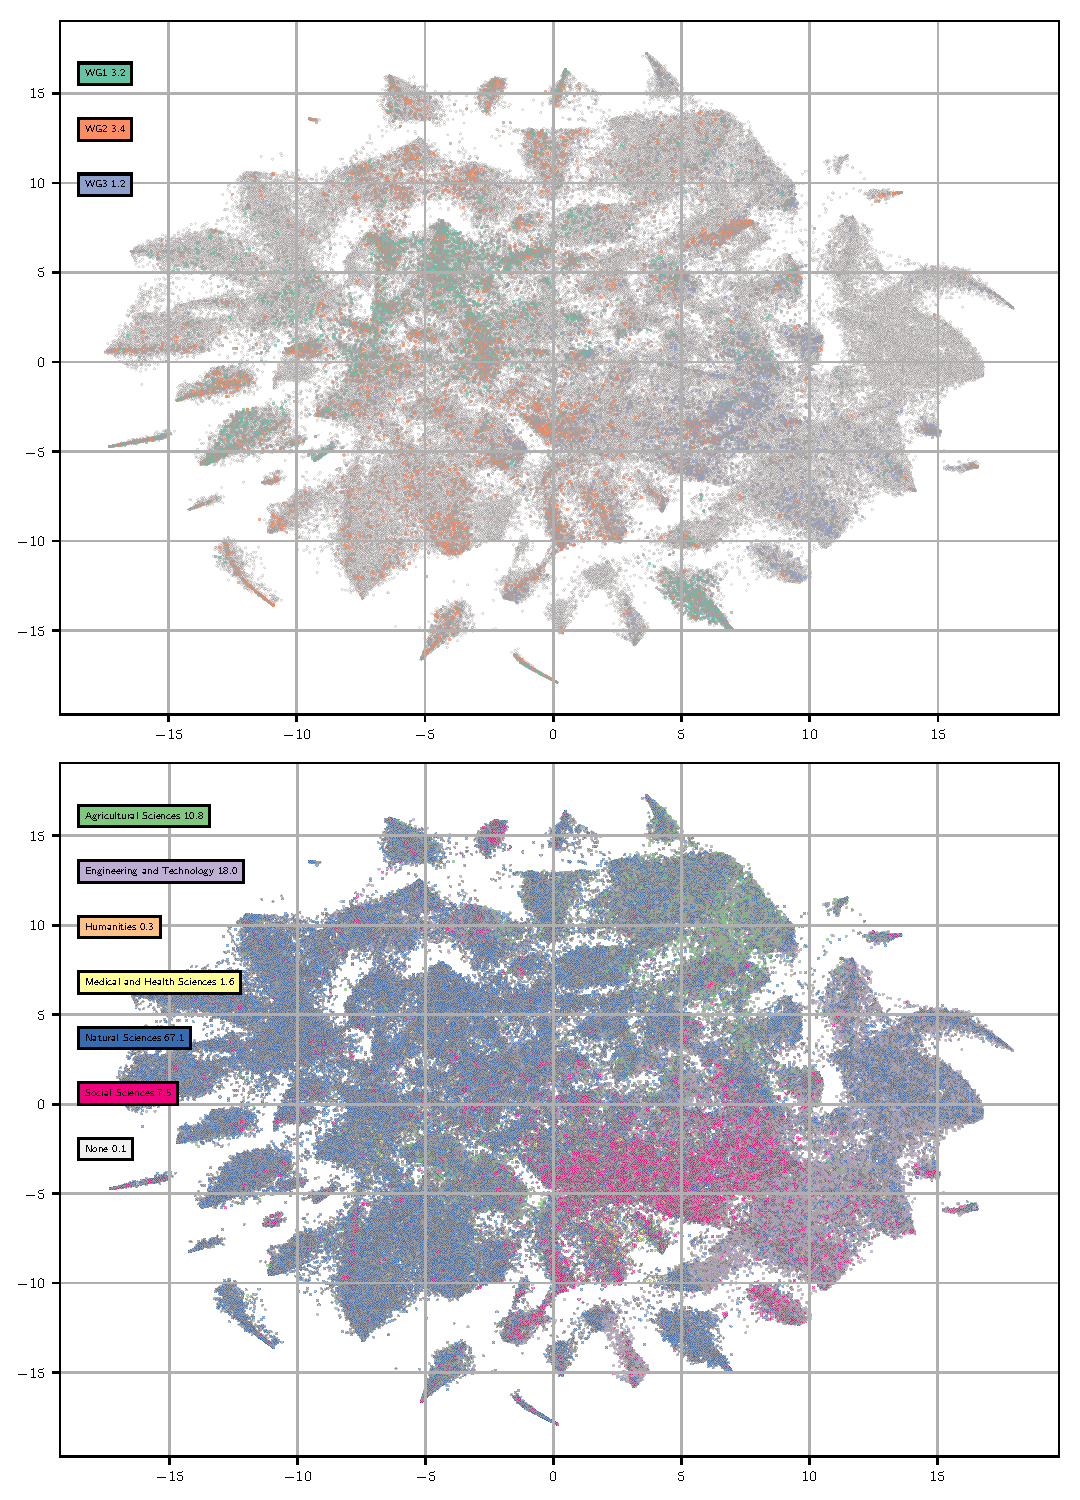
\includegraphics[width=1\linewidth]{tsne_results/plots/run_665_s_0_p200_double.pdf}
%		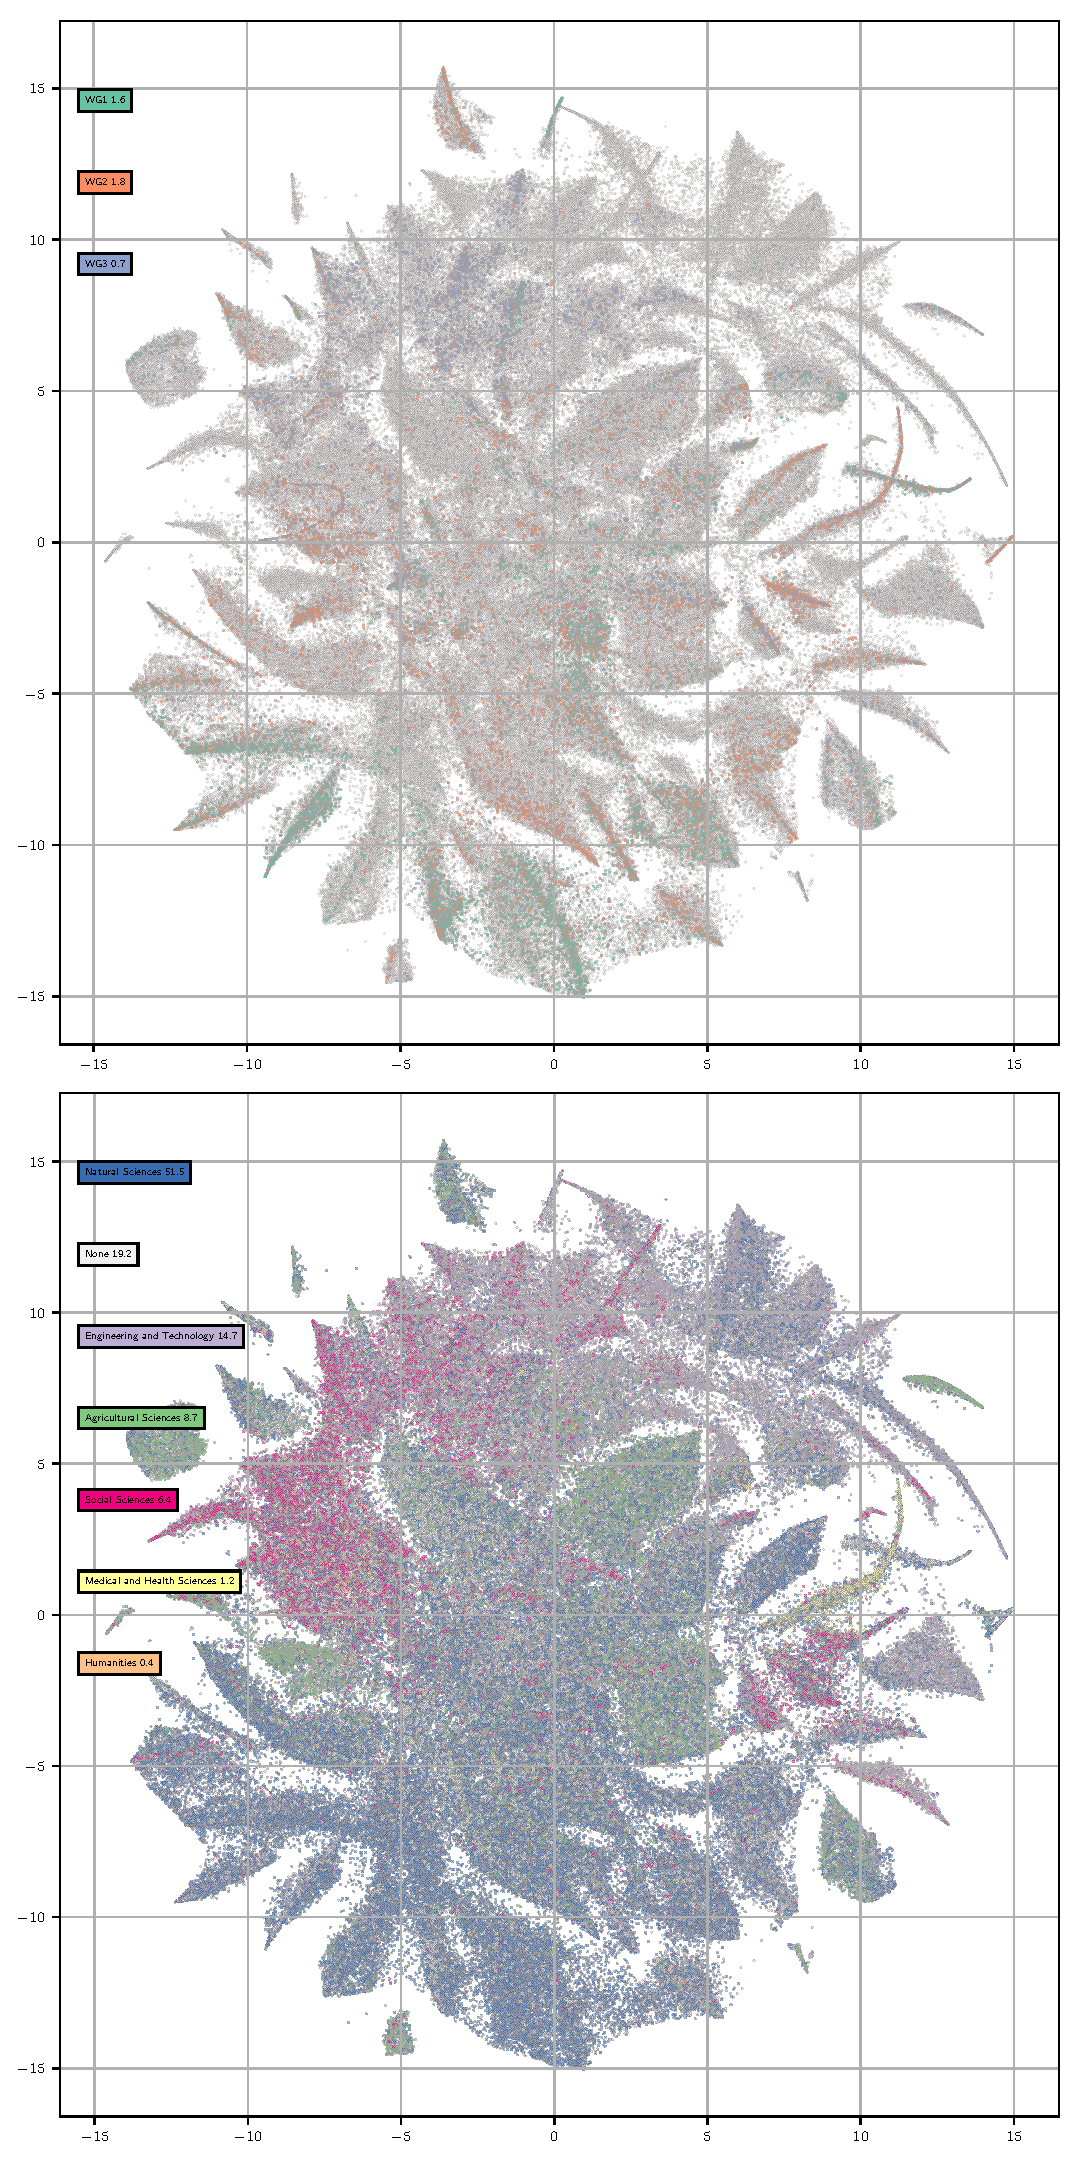
\includegraphics[width=0.85\linewidth]{tsne_results/plots/run_1275_s_0_p100_double.png}
%		\caption{A map of the literature on climate change. Document positions are obtained by reducing the topic scores to two dimensions via t-SNE Documents are coloured by working group citations (top) and web of science discipline category (bottom). See SI table for topic composition of each grid square}
%		\label{map-double}
%	\end{center}
%\end{figure}

\subsection{Topic structure of literature maps to broad disciplinary categories}

%\todo{Label some topics particularly representative of certain disciplines, and their growth with reference to below}

\begin{figure}[h!]
	\begin{center}
		%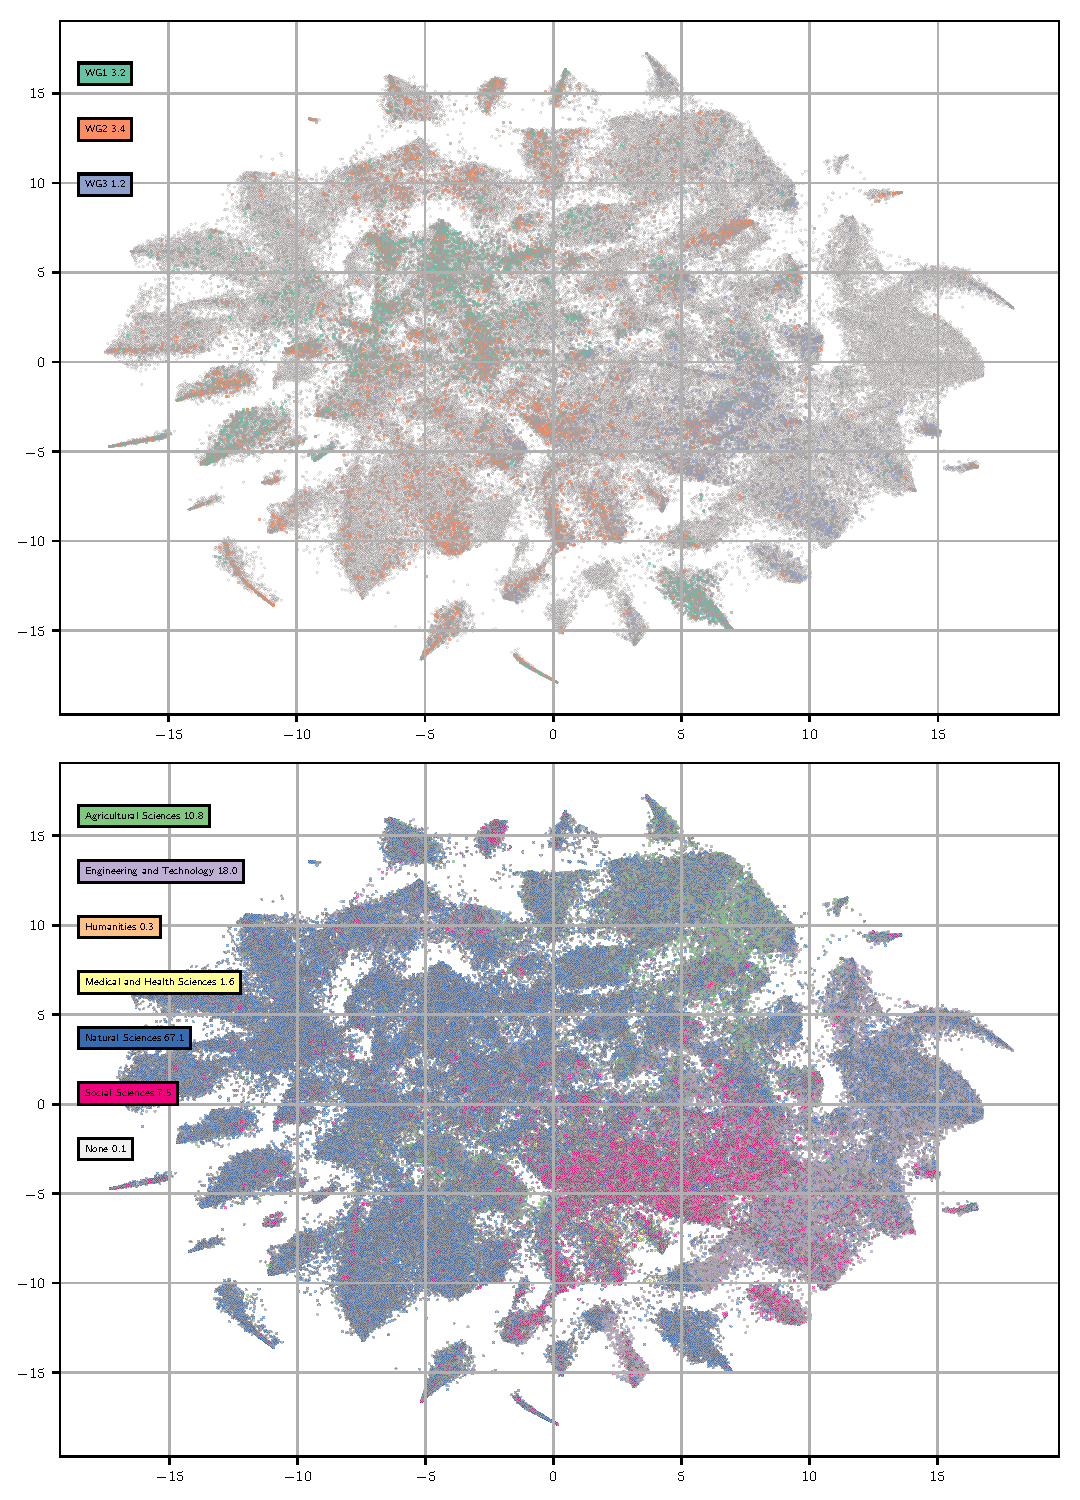
\includegraphics[width=1\linewidth]{tsne_results/plots/run_665_s_0_p200_double.pdf}
		\includegraphics[width=1\linewidth]{tsne_results/plots/run_1771_s_0_p200_all_topic_words_oecds.png}
		\caption{A map of the literature on climate change. Document positions are obtained by reducing the topic scores to two dimensions via t-SNE Documents are coloured by web of science discipline category. See SI table for topic composition of each grid square}
		\label{map-oecd}
	\end{center}
\end{figure}

\begin{itemize}
	\item The thematic structure of the topics reflects journal disciplinary categories. 
	\item Different disciplines clearly deal with different themes, although some topics are more interdisciplinary \todo{Show disciplinary entropy of topics in SI, give examples}
	%\item Medicine has the most specialized topic distribution  
	\item Topics in the south of the map (coal, oil, gas, cement, power) show a strong mix of social sciences and engineering
\end{itemize}

\bigskip

\subsection{Contrary to suggestions, the social sciences are over-represented in IPCC reports, while agricultural sciences and engineering are under-represented}


\citep{Bjurström2011} and \citep{Victor2015} point to an under-representation of social science literature within the IPCC, and a dominance of the natural sciences


\begin{figure}[h!]
	\begin{center}
		\includegraphics[width=0.85\linewidth]{plots/ipcc_representation/ipcc_rep_oecds_simplified.pdf}
		\caption{The representation within the IPCC of each discipline over time}
		\label{oecd_rep}
	\end{center}
\end{figure}

\begin{itemize}
	\item The natural sciences have always made up the greatest share of IPCC citations and documents about climate change
	\item The ratio of these two proportions tells us whether a certain discipline is over-represented or under-represented
	\item The natural are indeed slightly over-represented
	\item Although the Social sciences were under-represented in the past, by AR5, they were the most over-represented discipline

\end{itemize}

\bigskip

\subsection{Solution oriented topics have seen rapid growth, which has not been matched by coverage in the IPCC}

The topic model allows us to dig deeper into the content of the types of documents which are under-represented in the IPCC, as well as helping us understand how the thematic structure of the literature has developed.


%\todo{Just 4 subplots, mashing together ar1-2, and 3-4}
\begin{figure}[h!]
	\begin{center}
		%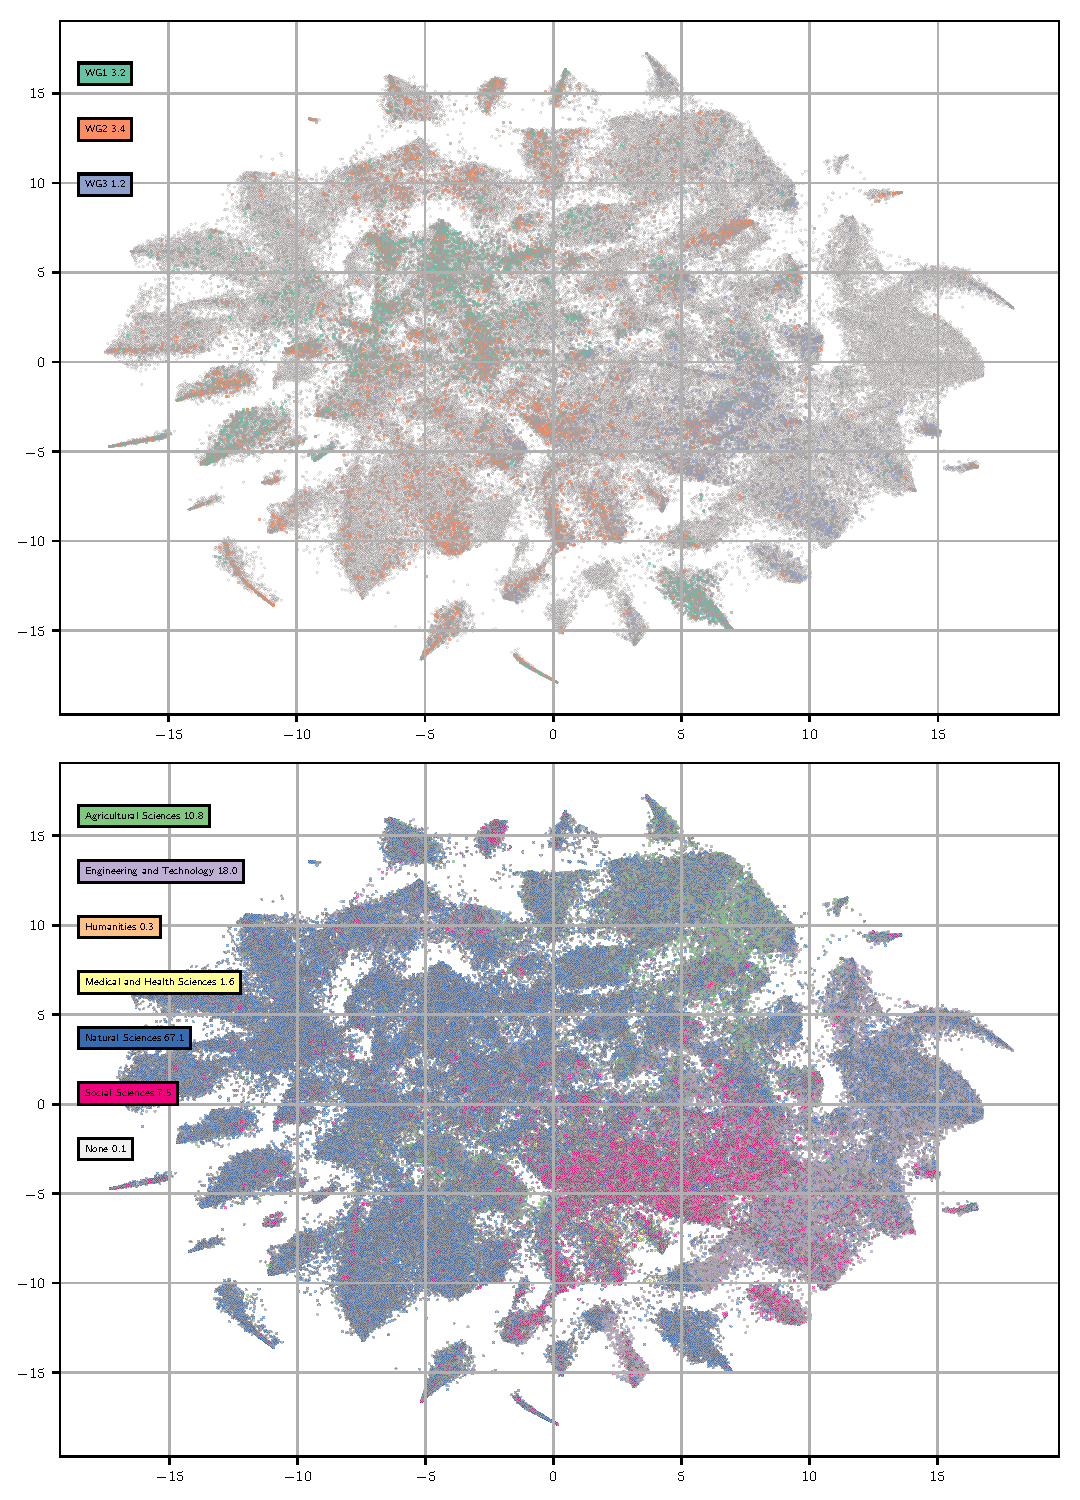
\includegraphics[width=1\linewidth]{tsne_results/plots/run_665_s_0_p200_double.pdf}
		\includegraphics[width=1\linewidth]{tsne_results/plots/run_1771_s_0_p200_evolution_4.png}
		\caption{A map of the literature on climate change. Document positions are obtained by reducing the topic scores to two dimensions via t-SNE Documents are coloured by working group citations. In each assessment period, the largest cluster of documents relating to each of the 10 fastest growing topics is outlined.}
		\label{map-evolution}
		
	\end{center}
\end{figure}

\begin{itemize}
	\item The thematic structure is also reflected in the division of labour between IPCC working groups. Documents cited by each working group appear in discrete parts of the map (which correspond also to the disciplinary structure)
	\item A number of different patterns of growth are visible. Adsorption was a fast growing topic in AR5, but had few IPCC citations, while risk and adaptation were fast growing, with many WGII citations

	%\item Some fast growing topics [e.g. health] are well represented in IPCC [WGII], whereas others (particularly on negative emissions) are not so well represented.
	
\end{itemize}

%\begin{figure}[h!]
%	\begin{center}
%		\includegraphics[width=0.85\linewidth]{example-image}
%		\caption{Optional figure, instead of above, one large wg map, with the topics below labelled}
%		\label{ipcc_rep}
%	\end{center}
%\end{figure}

\bigskip

\noindent By plotting each topic's newness and IPCC representation, we can dig down into the types of topics which are over or under represented

\begin{figure}[h!]
	\begin{center}
		\includegraphics[width=0.85\linewidth]{plots/ipcc_representation/ipcc_rep_new1771_all.pdf}
		\caption{The IPCC representation and age of the topics. Representation shows the log of the share of topic documents in IPCC citations divided by the share of topic documents among all documents. Assessment period occurence shows the assessment period in which the mean topic document was published}
		\label{ipcc_rep}
	\end{center}
\end{figure}

\begin{itemize}
	\item Those topics that deal with working group III issues (negative emissions, buildings) are in general fast growing and under-represented in IPCC reports
	%\item Some working group III topics (on scenarios, on policies, and on international trade and cross country comparisons) are however over-represented in IPCC reports [see SI]
	\item Working group I topics are in general older and better represented. 
	\item Of the newer topics that are well represented, many are on WG II issues 
	%\item Are WGII better at reflecting changes in the literature?
	%\item Another plot showing lines for each topic showing growth in literature and growth in ipcc?
\end{itemize}

Within working group III, those topics which have more citations from the social sciences are better represented (SI figure x.) These are general topics about policy options, and international politics. Those topics which are not well represented are on specific solutions, such as vehicles, buildings, and negative emissions. 

While there may be a need for more social science knowledge in IPCC assessments, this analysis makes it clear that this is rather a task for social scientists to produce more knowledge, than for the IPCC to reflect it better. 

Further, given Policymakers' demands for more solution-oriented knowledge, the IPCC may do well to make efforts to cover more of the literature on individual solutions.

It may be argued that the technical solution-oriented knowledge is not yet in a proper form for synthesis by the IPCC. Although this is not an argument made for WGII (where the relationship between social science percentage and IPCC coverage for topics is not found), it would then be a task for the social sciences to produce research on solution oriented topics: increasing, for example, the less than 5\% of the research on biochar that is published by social scientists.



\section{SI}
\begin{figure}[h!]
	\begin{center}
		\includegraphics[width=0.85\linewidth]{plots/run_1771_wgs_socsci.pdf}
		\caption{}
		\label{ipcc_rep}
	\end{center}
\end{figure}


\subsection{Glossary}


\noindent\textbf{ncep:} National Centers for Environmental Protection

\noindent\textbf{fco:} Fugacity of Carbon Dioxide

\noindent\textbf{pfc:} Perflourocompound
	
\noindent\textbf{otcs:} Open Top Chambers

\noindent\textbf{dtr:} Diurnal Temperature Range

\noindent\textbf{sres:} Special Report on Emissions Scenarios

\noindent\textbf{petm:} Paleocene Eocene Thermal Maximum

\noindent\textbf{amf:}  Arbuscular Mycorrhizal Fungal

\noindent\textbf{sf5cf3:} trifluoromethyl sulfur pentafluoride (A Potent Greenhouse Gas Identified in the Atmosphere, 2000)

\noindent\textbf{clc:} Chemical Looping Combustion

\noindent\textbf{cwd:} Coarse woody debris

\noindent\textbf{etm:} Enhanced Thematic Mapper (NASA satellite sensor)

\noindent\textbf{cmip5:} Coupled Model Intercomparison Project 5 (Starting 2008)

\noindent\textbf{cmip3:} Coupled Model Intercomparison Project phase 3 (2005-2006)

\noindent\textbf{mofs:} metal-organic frameworks (for CO2 storage)

\noindent\textbf{sdm:} statistical-dynamical model

\noindent\textbf{mmms:} Mixed Matrix Membranes (for CO2 capture)

\noindent\textbf{cop21:} 21 Conference of Parties (Paris 2015) 

\noindent\textbf{c3n4:} Carbon nitride (a synthetic nanomaterial used for hydrogen production)

\noindent\textbf{sdg:} Sustainable Development Goals

\noindent\textbf{indc:} Intended Nationally Determined Contributions

\begin{table}[h!]
	\scriptsize
	\begin{tabular}{lrrrrlr}
\toprule
{} &  ipcc\_share &     share &  representation &  primary\_wg &                                   title &   year\_av \\
\midrule
0  &    0.004058 &  0.004018 &        1.010164 &           3 &            \{urban, urbanization, rural\} &  4.972222 \\
1  &    0.003674 &  0.003661 &        1.003379 &           3 &                     \{city, plan, smart\} &  4.968750 \\
2  &    0.002319 &  0.005692 &        0.407461 &           3 &        \{building, construction, design\} &  4.930233 \\
3  &    0.003022 &  0.004487 &        0.673426 &           3 &             \{china, province, industry\} &  4.897436 \\
4  &    0.004142 &  0.008851 &        0.467975 &           3 &             \{material, waste, concrete\} &  4.813953 \\
5  &    0.003743 &  0.008900 &        0.420550 &           3 &         \{storage, reservoir, injection\} &  4.765957 \\
6  &    0.002805 &  0.010014 &        0.280143 &           3 &           \{reaction, catalyst, reactor\} &  4.727273 \\
7  &    0.010519 &  0.007718 &        1.362937 &           3 &           \{project, future, projection\} &  4.725000 \\
8  &    0.001641 &  0.004343 &        0.377916 &           3 &            \{soc, stock, organic-carbon\} &  4.693878 \\
9  &    0.002860 &  0.004431 &        0.645447 &           3 &                    \{vehicle, road, car\} &  4.684211 \\
10 &    0.005694 &  0.008783 &        0.648375 &           3 &           \{technology, cc, development\} &  4.660000 \\
11 &    0.003210 &  0.008343 &        0.384725 &           3 &              \{power, electricity, grid\} &  4.659574 \\
12 &    0.004129 &  0.008680 &        0.475662 &           3 &          \{process, solvent, absorption\} &  4.642857 \\
13 &    0.011922 &  0.009388 &        1.269943 &           3 &        \{country, international, income\} &  4.625000 \\
14 &    0.009222 &  0.013611 &        0.677533 &           3 &          \{system, performance, control\} &  4.620000 \\
15 &    0.009744 &  0.007007 &        1.390590 &           3 &          \{policy, government, national\} &  4.604167 \\
16 &    0.001903 &  0.005535 &        0.343928 &           3 &        \{coal, combustion, gasification\} &  4.576923 \\
17 &    0.005973 &  0.005985 &        0.997967 &           3 &            \{price, market, electricity\} &  4.571429 \\
18 &    0.002569 &  0.006206 &        0.413890 &           3 &              \{fuel, engine, combustion\} &  4.555556 \\
19 &    0.007430 &  0.012652 &        0.587273 &           3 &                \{energy, source, supply\} &  4.540000 \\
20 &    0.007932 &  0.007616 &        1.041498 &           3 &               \{cost, benefit, economic\} &  4.500000 \\
21 &    0.012278 &  0.006699 &        1.832801 &           2 &         \{adaptation, local, mitigation\} &  4.906977 \\
22 &    0.007655 &  0.004174 &        1.834058 &           2 &      \{vulnerability, index, resilience\} &  4.888889 \\
23 &    0.007639 &  0.007915 &        0.965149 &           2 &               \{disease, health, vector\} &  4.863636 \\
24 &    0.011768 &  0.006763 &        1.739972 &           2 &                \{risk, disaster, hazard\} &  4.767442 \\
25 &    0.005855 &  0.005478 &        1.068680 &           2 &                \{coral, reef, bleaching\} &  4.745098 \\
26 &    0.012762 &  0.015922 &        0.801515 &           2 &                   \{area, region, study\} &  4.737705 \\
27 &    0.003618 &  0.004426 &        0.817593 &           2 &              \{network, design, propose\} &  4.722222 \\
28 &    0.004257 &  0.006594 &        0.645509 &           2 &           \{habitat, fish, conservation\} &  4.714286 \\
29 &    0.006044 &  0.007850 &        0.769862 &           2 &     \{community, diversity, composition\} &  4.711111 \\
30 &    0.003077 &  0.004400 &        0.699417 &           2 &        \{irrigation, agricultural, crop\} &  4.666667 \\
31 &    0.007697 &  0.006230 &        1.235435 &           2 &               \{flood, flooding, damage\} &  4.660000 \\
32 &    0.007355 &  0.011205 &        0.656424 &           2 &             \{population, genetic, gene\} &  4.627451 \\
33 &    0.007961 &  0.006139 &        1.296844 &           2 &               \{extreme, event, weather\} &  4.621622 \\
34 &    0.008249 &  0.010310 &        0.800063 &           2 &                \{river, flow, discharge\} &  4.615385 \\
35 &    0.006453 &  0.009894 &        0.652212 &           2 &              \{production, product, lca\} &  4.608696 \\
36 &    0.002745 &  0.005076 &        0.540759 &           2 &                  \{wetland, marsh, peat\} &  4.600000 \\
37 &    0.021372 &  0.010701 &        1.997210 &           2 &              \{scenario, future, impact\} &  4.588235 \\
38 &    0.009649 &  0.010903 &        0.884979 &           2 &             \{ecosystem, grassland, net\} &  4.576923 \\
39 &    0.006615 &  0.008457 &        0.782182 &           2 &                    \{crop, yield, wheat\} &  4.574468 \\
40 &    0.022217 &  0.023637 &        0.939943 &           2 &       \{research, social, environmental\} &  4.566038 \\
41 &    0.001633 &  0.002769 &        0.589591 &           2 &           \{seed, germination, seedling\} &  4.558824 \\
42 &    0.007638 &  0.007042 &        1.084746 &           2 &                \{drought, index, severe\} &  4.553191 \\
43 &    0.008042 &  0.008349 &        0.963322 &           2 &              \{runoff, catchment, basin\} &  4.538462 \\
44 &    0.006931 &  0.006752 &        1.026497 &           2 &                  \{fire, burn, wildfire\} &  4.527273 \\
45 &    0.010619 &  0.009743 &        1.089913 &           2 &                    \{heat, wave, stress\} &  4.520833 \\
46 &    0.003965 &  0.007032 &        0.563803 &           2 &              \{biomass, stand, estimate\} &  4.519231 \\
47 &    0.004671 &  0.009894 &        0.472140 &           2 &               \{site, elevation, across\} &  4.517857 \\
48 &    0.012839 &  0.018694 &        0.686784 &           2 &           \{specie, distribution, range\} &  4.509434 \\
49 &    0.029153 &  0.017775 &        1.640145 &           2 &               \{change, response, shift\} &  4.436364 \\
50 &    0.007613 &  0.020954 &        0.363336 &           2 &              \{soil, content, microbial\} &  4.436364 \\
51 &    0.005960 &  0.007137 &        0.835032 &           2 &               \{vegetation, ndvi, index\} &  4.403509 \\
52 &    0.006156 &  0.007463 &        0.824883 &           2 &                    \{rice, paddy, field\} &  4.400000 \\
53 &    0.010491 &  0.013758 &        0.762548 &           2 &            \{forest, stand, disturbance\} &  4.400000 \\
54 &    0.004189 &  0.008951 &        0.468042 &           2 &                   \{lake, diatom, level\} &  4.385965 \\
55 &    0.005309 &  0.013352 &        0.397643 &           2 &                   \{plant, stress, grow\} &  4.381818 \\
56 &    0.005290 &  0.010154 &        0.521033 &           2 &                     \{tree, ring, stand\} &  4.375000 \\
57 &    0.005140 &  0.007852 &        0.654579 &           2 &                \{growth, rate, response\} &  4.362069 \\
58 &    0.012828 &  0.018330 &        0.699840 &           2 &              \{co2, mol, carbon-dioxide\} &  4.351852 \\
59 &    0.005615 &  0.012157 &        0.461877 &           2 &            \{sediment, erosion, deposit\} &  4.283333 \\
60 &    0.003613 &  0.009090 &        0.397449 &           2 &                     \{root, fine, shoot\} &  4.229508 \\
61 &    0.000331 &  0.000934 &        0.354604 &           1 &       \{biochar, amendment, application\} &  4.823529 \\
62 &    0.002146 &  0.006136 &        0.349778 &           1 &        \{adsorption, membrane, capacity\} &  4.818182 \\
63 &    0.007327 &  0.006128 &        1.195698 &           1 &                     \{wind, speed, wave\} &  4.708333 \\
64 &    0.014059 &  0.013316 &        1.055799 &           1 &                 \{scale, spatial, large\} &  4.687500 \\
65 &    0.010929 &  0.006738 &        1.622034 &           1 &              \{arctic, permafrost, thaw\} &  4.680851 \\
66 &    0.014972 &  0.008280 &        1.808290 &           1 &     \{uncertainty, estimate, projection\} &  4.666667 \\
67 &    0.017338 &  0.011734 &        1.477549 &           1 &           \{trend, station, significant\} &  4.551724 \\
68 &    0.009873 &  0.013702 &        0.720580 &           1 &                   \{data, use, estimate\} &  4.538462 \\
69 &    0.014492 &  0.010710 &        1.353111 &           1 &           \{land, surface, agricultural\} &  4.530612 \\
70 &    0.011837 &  0.016381 &        0.722589 &           1 &                 \{method, use, analysis\} &  4.511111 \\
71 &    0.014068 &  0.011336 &        1.241021 &           1 &            \{increase, effect, decrease\} &  4.481481 \\
72 &    0.019953 &  0.016658 &        1.197806 &           1 &   \{emission, greenhouse-gas, reduction\} &  4.472727 \\
73 &    0.011712 &  0.009366 &        1.250456 &           1 &            \{solar, radiation, activity\} &  4.463768 \\
74 &    0.039358 &  0.023349 &        1.685632 &           1 &           \{model, simulation, simulate\} &  4.462963 \\
75 &    0.039974 &  0.018618 &        2.147088 &           1 &               \{climate, future, global\} &  4.462963 \\
76 &    0.013584 &  0.011648 &        1.166208 &           1 &                     \{degree, day, warm\} &  4.461538 \\
77 &    0.019015 &  0.012243 &        1.553195 &           1 &         \{precipitation, annual, region\} &  4.454545 \\
78 &    0.008347 &  0.005916 &        1.410901 &           1 &                \{glacier, mass, balance\} &  4.446429 \\
79 &    0.011389 &  0.009026 &        1.261840 &           1 &               \{rainfall, monsoon, rain\} &  4.446429 \\
80 &    0.024706 &  0.019448 &        1.270381 &           1 &                \{temperature, air, warm\} &  4.444444 \\
81 &    0.031758 &  0.017706 &        1.793643 &           1 &                    \{sst, pacific, enso\} &  4.437500 \\
82 &    0.008400 &  0.007062 &        1.189491 &           1 &                    \{snow, cover, depth\} &  4.435484 \\
83 &    0.010006 &  0.014464 &        0.691740 &           1 &                    \{water, deep, vapor\} &  4.433962 \\
84 &    0.011541 &  0.012119 &        0.952267 &           1 &                     \{carbon, low, sink\} &  4.418182 \\
85 &    0.021681 &  0.014004 &        1.548168 &           1 &                      \{sea, level, rise\} &  4.400000 \\
86 &    0.014568 &  0.011804 &        1.234124 &           1 &                \{winter, season, summer\} &  4.382979 \\
87 &    0.009785 &  0.012267 &        0.797633 &           1 &          \{concentration, nutrient, doc\} &  4.357143 \\
88 &    0.014706 &  0.013420 &        1.095796 &           1 &                  \{year, period, annual\} &  4.354167 \\
89 &    0.006848 &  0.011702 &        0.585178 &           1 &                 \{gas, methane, hydrate\} &  4.350877 \\
90 &    0.010142 &  0.014490 &        0.699914 &           1 &                 \{record, holocene, cal\} &  4.349206 \\
91 &    0.005465 &  0.011081 &        0.493212 &           1 &                 \{delta, isotope, value\} &  4.349206 \\
92 &    0.024719 &  0.010410 &        2.374563 &           1 &             \{cloud, aerosol, radiative\} &  4.315789 \\
93 &    0.028157 &  0.013651 &        2.062692 &           1 &              \{ocean, circulation, deep\} &  4.301587 \\
94 &    0.018071 &  0.010357 &        1.744728 &           1 &                       \{ice, sheet, sea\} &  4.301587 \\
95 &    0.008723 &  0.012357 &        0.705902 &           1 &            \{flux, measurement, surface\} &  4.281250 \\
96 &    0.002649 &  0.006194 &        0.427682 &           1 &   \{n2o, denitrification, nitrous-oxide\} &  4.228070 \\
97 &    0.005092 &  0.007353 &        0.692544 &           1 &               \{ch4, methane, oxidation\} &  4.226415 \\
98 &    0.003659 &  0.013634 &        0.268363 &           1 &  \{leaf, photosynthetic, photosynthesis\} &  4.177419 \\
99 &    0.017143 &  0.008313 &        2.062174 &           1 &    \{ozone, stratospheric, tropospheric\} &  4.164384 \\
\bottomrule
\end{tabular}

	\caption{Topics and their representation}
	\label{top-topics}
\end{table}	

%\begin{table}[h!]
%	\scriptsize
%	\begin{tabular}{p{1.9cm} p{3cm} p{7.5cm} r}
\toprule
                      title &                                                                            top words &                                                                                                                                                                                                                                                                top docs &   share \\
\midrule
      climat, chang, impact &          [climat, chang, impact, respons, futur, effect, shift, sensit, affect, may] &                                                                                                                                                  \parbox[t]{7.5cm}{Climate oscillations and changes over Russia; \\World Regionalization of Climate Change (1961-2010)} &  2.73\% \\
     soil, moistur, microbi &       [soil, moistur, microbi, organ, respir, content, miner, depth, matter, efflux] &                                                                                    \parbox[t]{7.5cm}{PARTITIONING OF SOIL RESPIRATION IN A FIRST ROTATION BEECH PLANTATION; \\Responses of soil respiration to N fertilization in a loamy soil under maize cultivation} &  2.73\% \\
       emiss, reduct, reduc &      [emiss, reduct, reduc, greenhous, factor, total, estim, inventori, nox, measur] &                                                                                                             \parbox[t]{7.5cm}{China's CH4 and CO2 emissions: Bottom-up estimation and comparative analysis; \\Monitoring total emissions from industrial installations} &  2.21\% \\
   carbon, dioxid, sequestr &   [carbon, dioxid, sequestr, sink, organ, cycl, storag, stock, terrestri, atmospher] &                             \parbox[t]{7.5cm}{Interpreting carbon-isotope excursions: carbonates and organic matter; \\PARTICULATE FLUXES OF CARBONATE AND ORGANIC-CARBON IN THE OCEAN - IS THE MARINE BIOLOGICAL-ACTIVITY WORKING AS A SINK OF THE ATMOSPHERIC CARBON} &  1.74\% \\
      temperatur, air, mean &  [temperatur, air, mean, surfac, minimum, maximum, daili, increas, effect, degreesc] &                                                                                                     \parbox[t]{7.5cm}{Observed changes in shallow soil temperatures in Northeast China, 1960-2007; \\Beyond the Mean: Biological Impacts of Cryptic Temperature Change} &  1.71\% \\
      record, dure, glacial &       [record, dure, glacial, reconstruct, last, period, holocen, event, late, core] &                                                           \parbox[t]{7.5cm}{HIGH-RESOLUTION CLIMATE RECORDS FROM THE NORTH-ATLANTIC DURING THE LAST INTERGLACIAL; \\HIGH-RESOLUTION CLIMATIC INFORMATION FROM SHORT FIRN CORES, WESTERN DRONNING MAUD LAND, ANTARCTICA} &   1.7\% \\
     speci, distribut, rang &          [speci, distribut, rang, rich, invas, nich, predict, extinct, shift, abund] &                               \parbox[t]{7.5cm}{Northward range extensions of some mesopelagic fishes in the Northeastern Atlantic; \\Natural occurrence and backwater infection of C-4 plants in the vegetation of the Yangtze hydropower Three Gorges Project region} &   1.7\% \\
 increas, concentr, decreas &   [increas, concentr, decreas, effect, atmospher, doc, result, organ, nutrient, may] &                                                          \parbox[t]{7.5cm}{TERRESTRIAL HIGHER-PLANT RESPONSE TO INCREASING ATMOSPHERIC [CO2] IN RELATION TO THE GLOBAL CARBON-CYCLE; \\Hydrological response to climate change in the Black Hills of South Dakota, USA} &  1.61\% \\
      forest, tropic, stand &       [forest, tropic, stand, deforest, disturb, stock, boreal, redd, harvest, wood] &  \parbox[t]{7.5cm}{Spatially explicit estimates and temporal changes of forest tree biomass in a typical department of forest management, Turkey; \\Analysis of the changes in forest ecosystem functions, structure and composition in the Black Sea region of Turkey} &  1.56\% \\
    energi, renew, consumpt &        [energi, renew, consumpt, effici, demand, save, sector, sourc, industri, use] &                                                                                                                                       \parbox[t]{7.5cm}{Energy issues and energy priorities; \\Energy efficiency and CO2 emissions in Swedish manufacturing industries} &  1.56\% \\
\bottomrule
\end{tabular}

%	\caption{Top 10 topics in climate change literature}
%	\label{top-topics}
%\end{table}

\bibliography{Mendeley}	

\end{document}